\begin{figure}[htbp]
\centering
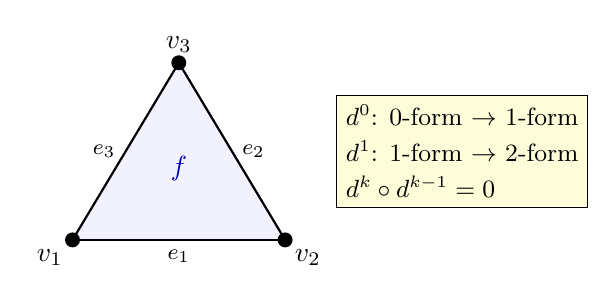
\begin{tikzpicture}[scale=0.9]
  \coordinate (v1) at (0,0);
  \coordinate (v2) at (3,0);
  \coordinate (v3) at (1.5,2.5);
  \fill[blue!5] (v1)--(v2)--(v3)--cycle;
  \draw[thick] (v1)--(v2) node[midway,below,font=\footnotesize] {$e_1$};
  \draw[thick] (v2)--(v3) node[midway,right,font=\footnotesize] {$e_2$};
  \draw[thick] (v3)--(v1) node[midway,left,font=\footnotesize] {$e_3$};
  \fill (v1) circle (3pt) node[below left] {$v_1$};
  \fill (v2) circle (3pt) node[below right] {$v_2$};
  \fill (v3) circle (3pt) node[above] {$v_3$};
  \node[blue!70!black] at (1.5,1) {$f$};
  \node[draw,rectangle,fill=yellow!15,font=\small,align=left] at (5.5,1.25) {
    $d^0$: 0-form $\to$ 1-form\\[2pt]
    $d^1$: 1-form $\to$ 2-form\\[2pt]
    $d^k \circ d^{k-1} = 0$
  };
\end{tikzpicture}
\caption{Discrete exterior derivative: $d^0$ maps vertex values to edge differences; $d^1$ maps edge values to face circulations.}
\label{fig:exterior_derivative}
\end{figure}
